% mycsrf 'for beeing included' snippet template
%
% (c) Karsten Reincke, Frankfurt a.M. 2012, ff.
%
% This text is licensed under the Creative Commons Attribution 3.0 Germany
% License (http://creativecommons.org/licenses/by/3.0/de/): Feel free to share
% (to copy, distribute and transmit) or to remix (to adapt) it, if you respect
% how you must attribute the work in the manner specified by the author(s):
% \newline
% In an internet based reuse please link the reused parts to mycsrf.fodina.de
% and mention the original author Karsten Reincke in a suitable manner. In a
% paper-like reuse please insert a short hint to mycsrf.fodina.de and to the
% original author, Karsten Reincke, into your preface. For normal quotations
% please use the scientific standard to cite
%




\subsubsection{Ptolemaic ($\bigstar$)}

\label{Ptolemaic}\acc{Ptolemaic} wird auf seiner Homepage -- sternenreich -- als
ein Programm zur Visualisierung und Untersuchung tonaler Musik offeriert, die
bei der Analyse \enquote{of all types of Western music} helfen könne und dazu
etablierte analytische Techniken nutze, \enquote{[\ldots] including tonal
functional analysis (Harrison 1994) [\ldots]}.\footcite[vgl.][\nopage
wp]{Ptolemaic2016a} Das Java-Programm wird als Paket zum Download angeboten, das
darin enthaltene \acc{jar}-File kann mit einem simplen \texttt{java -jar
Ptolemaic.jar} gestartet werden.\footcite[vgl.][\nopage wp]{Ptolemaic2016b} Es
liest \acc{MusicXML}-Dateien ein und exportiert \acc{seq}-Files.

Unsere Referenzkadenz II vermag \acc{Ptolemaic} in der \acc{MusicXML}-Version
erfolgreich zu laden, die \acc{Canorus} exportiert, nicht ohne allerdings das
angebliche Fehlen einer \enquote{tonicization} anzumahnen. Die
\acc{MusicXML}-Version der Refrenzkadenz II, die wir deshalb aus \acc{MuseScore}
heraus 'ersatzweise' exportiert haben, kann \acc{Ptolemaic} überhaupt nicht mehr
öffnen: es scheint dabei in eine Schleife zu geraten. Nach dem Einlesen der
Referenkadenz II bietet \acc{Ptolemaic} zwei Fenster an. Das eine enthält eine
Visualisierung der Töne in Form von Balken, das andere eine daraus abgeleitete
harmonische Analyse:

\begin{center}
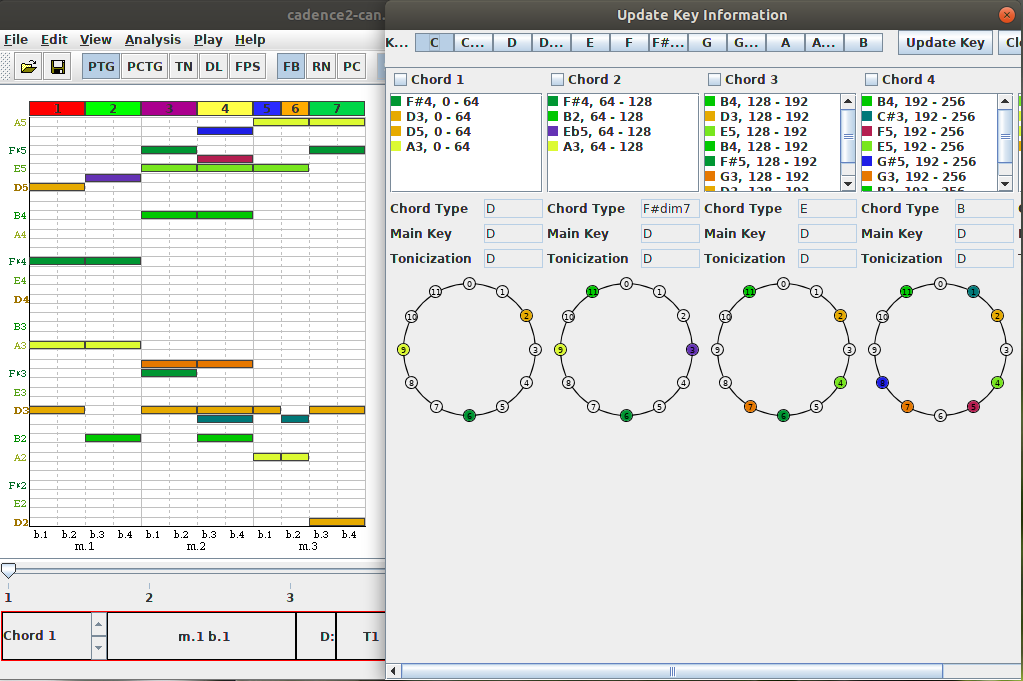
\includegraphics[width=0.9\textwidth]{frontends/ptolemaic/ptolemaic-2-win-300dpi.png}
\end{center}

Auch wenn \acc{Ptolemaic} über das Menue noch andere Analysen anbietet,
generiert es keine 'Noten', die man in einem \LaTeX-Text einbetten könnte, nicht
einmal als Bild. Außerdem erlaubt es vorderhand nicht, seine Analyseergebnisse
textuell zu exportieren. Von daher bietet \acc{Ptolemaic} hier wirklich keine
Unterstützung -- weder so, noch so.\footnote{Dass wir \acc{Ptolemaic} deshalb
nur einen Stern geben, ist in gewisser Hinsicht ungerecht: Man kann diesem
Programm kaum wirklich vorwerfen, unsere Ziele nur mangelhaft umgesetzt zu
haben. Es ist ja nur dadurch in unseren Blick geraten, dass es in der
MusicXML-Softwareseite gelistet wird (\cite[vgl.][\nopage
wp]{MusicXML2018b}). \acc{Ptolemaic} selbst ist gar nicht angetreten, den
Notendsatz zu unterstützen. Und da es das tut, was es wirklich tun will, wären 3
Sterne eigentlich angemessen. Wir belassen es trotzdem bei einem, weil es
gelegentlich abstürzt, Funktionen nicht ausführt und nicht bekennt, ob es nun
Open-Source-Software ist oder nicht.}

% this is only inserted to eject fault messages in texlipse
%\bibliography{../bib/literature}
